% !TEX root = paper.tex
\documentclass{article}
\usepackage[margin=1in]{geometry} % Adjust document margins
\usepackage{lipsum} % Dummy text
\usepackage{multicol} % Multi-column layout for the body
\usepackage[hidelinks]{hyperref}
\usepackage{graphicx}
\usepackage{caption}
\usepackage{tikz}
\usepackage{float}
\graphicspath{ {../images/} }


\title{Knowledge and Story Comprehension}
\author{Eduardo Badillo\thanks{UC Berkeley, Email: eduardo.badillo@berkeley.edu} \and Geronimo Walker\thanks{UC Berkeley, Email: 
geronimowalker@ischool.berkeley.edu} \and   Svein Gonzalez\thanks{UC Berkeley, Email: 
sggonzal@ischool.berkeley.edu}}
\date{\today}

\begin{document}

\maketitle

\begin{abstract}
\noindent % Align the abstract with the document's margin
It has been demonstrated that pre-trained language models have a good performance on numeric, and common-sense reasoning tasks with little or no fine-tunning needed. This performance is further enhanced when more context or knowledge of the input is provided to the model at the moment of inference; for it enables the model to leverage the knowledge it already contains from its pretraining and use it more effectively on downstream tasks. In this paper we study the impact of incorporating additional knowledge, with different structures and retrieval techniques, on tasks that require both reasoning and comprehension (ClozeStory Dataset) to determine a correct ending of a story. Our code is available at \href{https://github.com/sveinerss/w266_project}{Github}.
\end{abstract}

\begin{multicols}{2}
\section{Introduction}
There are two main ways in which task performance can be enhanced in pre-trained language models, by incorporating knowledge and by fine-tunning. The latter has shown that larger and larger models with fine-tunning diminish the need to integrate auxiliary knowledge (Khashabi et al., 2020; Lourie et al., 2021). Yet, incorporating knowledge on top of large-scale models (Liu et al. 2022) has shown a marked improvement on performance when no fine-tunning is involved. Suggesting that the models are able to exploit more effectively their pre-training knowledge when additional task-relevant information is provided. 

Obtaining and encoding relevant, contextual information isn't trivial. There might not be enough quality data for the task, and the way it is retrieved from the external knowledge structure and paired with the relevant keywords or entities in each sample must be also be thought of. 
The methods we will be using are knowledge graphs (Aglionbi et al. 2022) and knowledge prompting (Liu et al. 2022). We will add the relevant knowledge contained in each on top of pre-trained models, without fine-tunning to test whether their inclusion amounts to an increased performance on the story comprehension task. These approaches have been used on common-sense, numeric reasoning tasks where the query or question is configured in a syllogistic manner. But its usefulness on comprehension datasets, where samples have no straightforward outcomes, has yet to be tested. As baseline we will be using the models without knowledge structures, and standalone models (models without pre-training). 

\section{Prompt-based Knowledge}
\lipsum[3-4]

\section{Triples}
Triples are dependency representations of sentences. For example, take the sentence “David noticed he had put on a lot of weight recently", using Spacy, we can generate triples, 
most commonly Subject-Verb-Object (SVOs), to represent the sentence with the most relevant context and information. Drawing inspiration from 
Aglinoby and Teugel (2022), where graph representations of possible answers to questions are used to determine the highest ranking answer, our model will use 
extracted triples from the sentences comprising a story and compute a cosine similarity between the triples and two possible endings. Extracted 
triples are initially captured by a simple approach, speech tagging identification.

\begin{figure}[H]
    \centering
    \begin{tikzpicture}
        \node at (0,0) {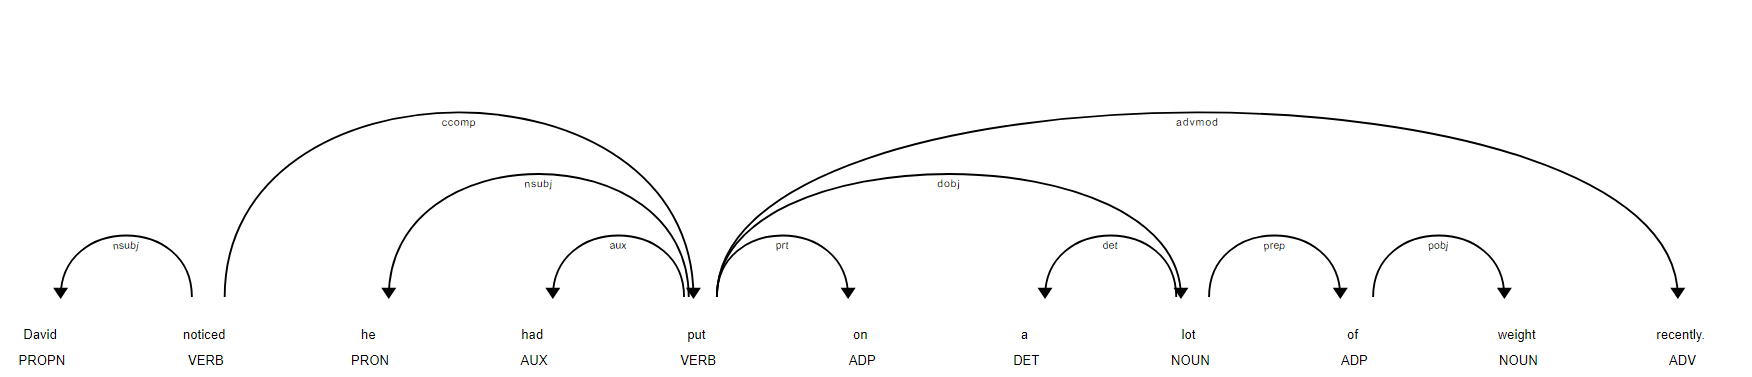
\includegraphics[width=8cm]{spacy.png}};
    \end{tikzpicture}
    \caption{Spacy Dependency Example}
\end{figure}

Using SPACY, we parse through all our sentences capturing words that are labeled "ROOT" (for verb), "nsubj" (for subject), or "dobj"/"pobj" (for object) 
into our SVO triples. It is important to note that "ROOT" can be a successful tag for verbs, but isn't a guarantee. As noted in Figure 1, certain words 
such as "put" are stronger central nodes than others since they share more dependencies.  This will be important to improve upon to optimally capture 
significant SVOs.

After generating SVOs, one for each story sentence, we use a bert model to generate cosine similarities for our different endings. We do so by
tokenizing our SVOs then running them through a bert model to obtain a mean pooled output for each triple. The story endings are treated the same.
Next we compute a cosine similarity between all the story sentences and the two possible endings (Figure 2). The initial attempt to use triples hasn't yieled
 remarkable results, only presenting a 50 percent accuracy.

\begin{figure}[H]
    \centering
    \begin{tikzpicture}
        \node at (0,0) {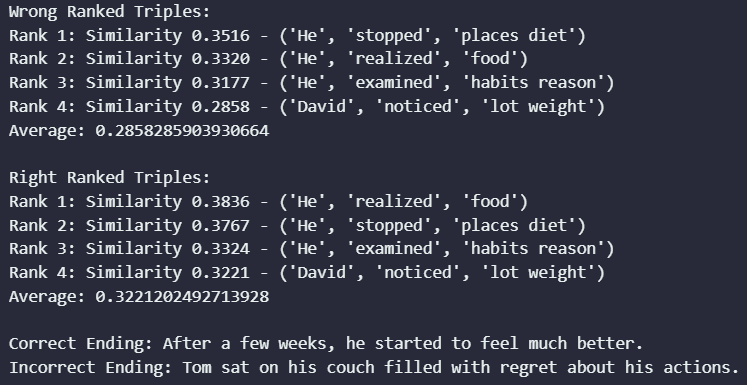
\includegraphics[width=8cm]{Cosine_Similarity.png}};
    \end{tikzpicture}
    \caption{Consine Similarity}
\end{figure}

However, the next models will investigate triples with better selection and ordering of the triples. Currently, all triples are weighed evenly 
when the cosines are averaged (Figure 2). The next model iteration will note the ending triples of the story more using a BertSeqtoSeq model. 

\end{multicols}

\end{document}

